\section{Non Equilibrium Normal and Oblique shock-wave forms}
Before starting the current, let us list out some assumptions that are formulated,
\begin{itemize}
\item[--] The temperature in the flowfield is high enough to cause chemical reactions within the flow.
\item[--] A strong shock wave is present in the flow.
\end{itemize}
The shock front, that is the thin region that is present where large gradient of velocity temperate and pressure occur which conclusively involves the viscosity and thermal conduction of the flow, which is called as shock wave in equilibrium flow or calorifically perfect gas, we assumed the flow in the front and back were uniform and discontinuities continued only through the shock of no more than few mean free path thickness.

In non-equilibrium flow, when the fluid element moves, all chemical reactions takes place at a finite rate because of the shock front which is too thin and the mean free path is very less with lesser number of collisions, hence if you recall the concept of frozen flow, the same concept is applied over here and therefore is essential in calculation of the chemical reaction that are occurring in the flow. Now all the properties behind the shock front are considered to be frozen flow properties. In downstream, as the fluid traverses, the finite reactions takes place, and the flow properties relaxes towards the equilibrium values. As result of all of these phenomenon, the shock wave now associated with the shock front and the non-equilibrium region behind where the flow properties are changing due to the flow properties.

For example, consider figure 3, assume a gas that is diatomic nitrogen which is pure which is present in front of the shock wave

\begin{figure}[ht]

\centering
  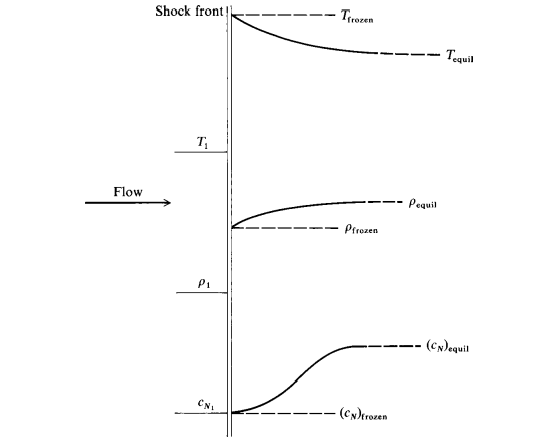
\includegraphics[width=0.7\linewidth]{images/schematic_n2.png}
  \caption{Chemically reacting Non-Equilibrium flow behind a normal shock wave}
  \label{fig:boat1}
\end{figure}

The properties, in front of the shock front, just next to the initial node or point follows the frozen flow results the back of shock front is calculated from the isentropic relation or the frozen flow relation and if observed properly, the properties are same up to some extent in and downstream of the shock front, the rest of the flow features, are predicted using non-equilibrium flow relations because of high temperature, the gas has already been disassociated or ionized. In the above figure, c(N) increases and the temperature and density downstream of the shock front increases and decreases respectively, since the reactions are all endothermic and therefore will reach the equilibrium values later downstream.

Till here, we are assuming the flow is one-dimensional and steady, the equations that are assuming are

Global Continuity equation \vspace{3mm}
\[ \rho du + u d\rho = 0\]

Momentum \vspace{3mm}
\[dp =-p u du\]

Energy \vspace{3mm}
\[dh_0 = 0\]

Species Continuity \vspace{3mm}
\[u dc_i = \frac{w_i}{\rho} dx\]


\begin{figure}[ht]

\centering
  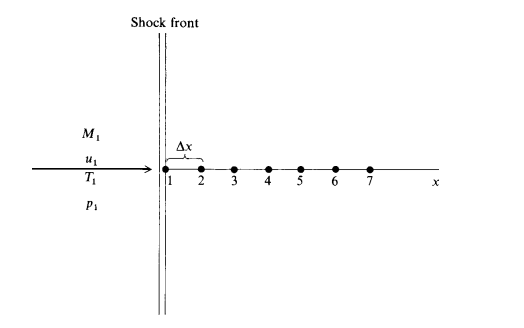
\includegraphics[width=0.7\linewidth]{images/numerical_method.png}
  \caption{Schematic of grid points for numerical solution of non-equilibrium normal shock flows}
  \label{fig:boat1}
\end{figure}

The flow field properties that are present behind the shock become a function of distance which makes the procedure easier to solve, since such type of flow problems can be easily done by standard numerical technique known as Runge-Kutta technique.

Consider figure 4, the initial conditions at point 1 are said to be frozen flow conditions and are obtained from isentropic flows,(assuming calorifically perfect gas) the chemical composition of the shock is the same the chemical composition of the shock at point 1.

Caution, the distance delta X must be chosen based on the rate of reaction that are occurring in the flow. If the rate of the reaction are fast, the delta x must be considered very small and a higher order numerical technique must be chosen.The stiff equation which often lead to instabilities in the equations are caused by species continuity equation because of the above phenomenon.

Marrone has conducted some experiments of non equilibrium flow on air at Mach number M = 12.28, which tends to reach temperatures very high and since the fluid is air, oxygen dissociated but Nitrogen partially dissociated and monotonously approached equilibrium after 10 cm downstream of the shock front.
As observed here, the fluid properties tend to vary from frozen to equilibrium ends. The species NO, increases at frozen values and overshoots when it reaches equilibrium value and then reached equilibrium and when observed temperature decreases and density increases behind the shock front.

\begin{figure}[ht]

\centering
  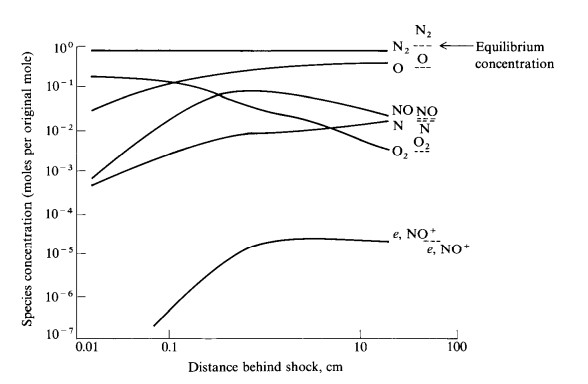
\includegraphics[width=0.7\linewidth]{images/species_dissociation.jpg}
  \caption{Distributions of the chemical species for the non equilibrium flow through
a normal shock wave in air}
  \label{fig:boat1}
\end{figure}

\begin{figure}[ht]

\centering
  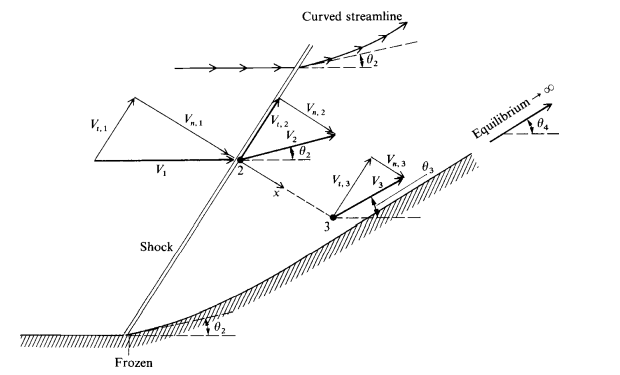
\includegraphics[width=0.7\linewidth]{images/oblique_shock.png}
  \caption{Geometry for non equilibrium flow behind a straight oblique shock
wave.}
  \label{fig:boat1}
\end{figure}

Let us start with the second part of this chapter, Non-Equilibrium flow around an oblique shock wave, Assume x is the distance between downstream of the shock front measured  perpendicular to the front. If you consider the moment part of the flow, it is understood that the tangential component of the velocity is preserved across the shock is constant everywhere behind the shock front whereas, the normal component of the momentum equation varies all along the direction. This assessment can be proved since the oblique shock properties based on an upstream velocity perpendicular to the shock front one which a constant tangential composed in imposed on the flow.

\begin{figure}[ht]

\centering
  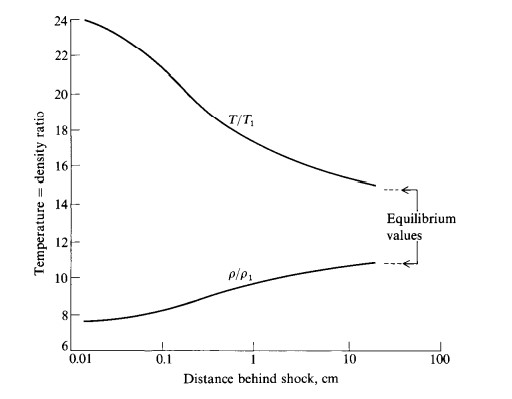
\includegraphics[width=0.7\linewidth]{images/distance_behind hsock.jpg}
  \caption{ Distributions of the temperature and density for the non equilibrium flow
through a normal shock wave in air.}
  \label{fig:boat1}
\end{figure}

From figure 7, it is understood that the density behind the shock front increases

In conclusion, the streamlines in the non equilibrium flow behind the oblique shock front are generally curved and continually  increase the deflection angle until equilibrium conditions are met far downstream of the shock wave. In order for the oblique shock remain straight in the downstream of the shock, the compression corner must be created in such a way that, after the flow crossed the shock front, that is frozen flow, must curve upward until the equilibrium conditions are reached far in the downstream.

\begin{figure}[ht]

\centering
  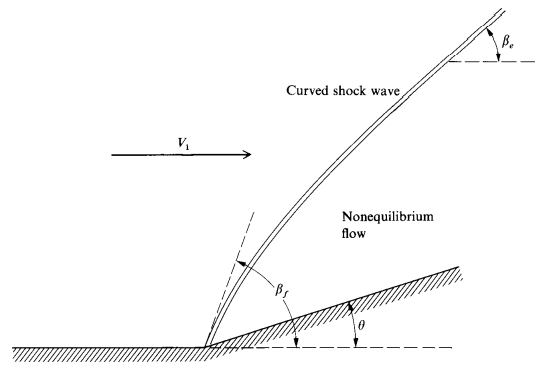
\includegraphics[width=0.7\linewidth]{images/compression_corner2.png}
  \caption{  Schematic of non equilibrium flow over a compression corner.}
  \label{fig:boat1}
\end{figure}

Consider the compression corner from figure 8, for such low angles, the oblique shock will remain curved, the wave angle at the start is considered to be frozen flow, and second angle is when is flow is in equilibrium state.

In conclusion, the non equilibrium flow depends on the distance from the normal shock. A term term arrives from such flows which is called Dimension scale, that is the non equilibrium length scale that is required to cool down or for the gas to settle to equilibrium conditions.

In conclusion let us trace the dimension scale for normal an d 30 deg oblique shock wave distance.

the relaxation distances behind a normal shock for T, Xo, and XN are
plotted vs free-stream Mach number, where the upstream conditions at each
Mach number correspond to the lower flight trajectory shown in figure 9 for a
trans-atmospheric vehicle in figure 10

if observed the nonequilibiurm distance are way less when compared oblique shock and this because of the higher temperatures that are obtained yield very high relaxation rated when compared to oblique shock waves.
and this is the major conclusion in which blunt body are majorly considered in re-entry scenarios and therefore the dimension scale is reduced and therefore in crease the quality of the material 
\begin{figure}[ht]

\centering
  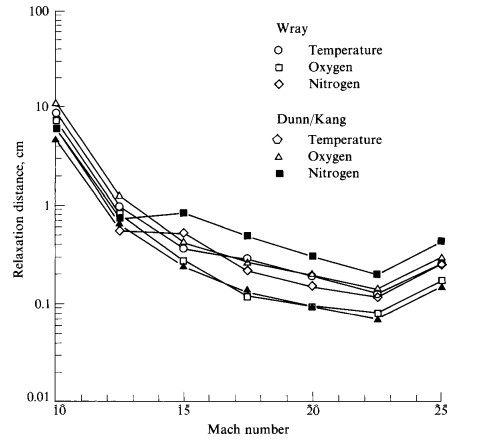
\includegraphics[width=0.5\linewidth]{images/normal shock relaxation distance.jpg}
  \caption{Nonequilibrium length scales behind a normal shock wave, following the
lower trajectory }
  \label{fig:boat1}
\end{figure}

\begin{figure}[ht]

\centering
  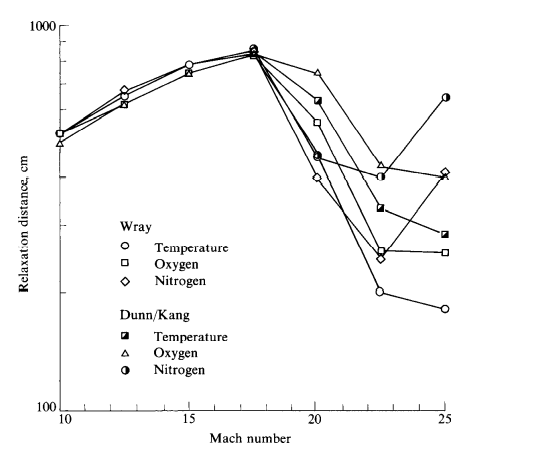
\includegraphics[width=0.7\linewidth]{images/oblique shock relation distance.png}
  \caption{  Nonequilibrium length scales behind a 30-deg oblique shock wave,
following the lower trajectory}
  \label{fig:boat1}
\end{figure}